\documentclass[12pt,twoside]{article}
\usepackage[dvipsnames]{xcolor}
\usepackage{tikz,graphicx,amsmath,amsfonts,amscd,amssymb,bm,cite,epsfig,epsf,url}
\usepackage[hang,flushmargin]{footmisc}
\usepackage[colorlinks=true,urlcolor=blue,citecolor=blue]{hyperref}
\usepackage{amsthm,multirow,wasysym,appendix}
\usepackage{array,subcaption} 
% \usepackage[small,bf]{caption}
\usepackage{bbm}
\usepackage{pgfplots}
\usetikzlibrary{spy}
\usepgfplotslibrary{external}
\usepgfplotslibrary{fillbetween}
\usetikzlibrary{arrows,automata}
\usepackage{thmtools}
\usepackage{blkarray} 
\usepackage{textcomp}
\usepackage[left=0.8in,right=1.0in,top=1.0in,bottom=1.0in]{geometry}

%% Probability operators and functions
%
% \def \P{\mathrm{P}}
\def \P{\mathrm{P}}
\def \E{\mathrm{E}}
\def \Var{\mathrm{Var}}
\let\var\Var
\def \Cov {\mathrm{Cov}} \let\cov\Cov
\def \MSE {\mathrm{MSE}} \let\mse\MSE
\def \sgn {\mathrm{sgn}}
\def \R {\mathbb{R}}
\def \C {\mathbb{C}}
\def \N {\mathbb{N}}
\def \Z {\mathbb{Z}}
\def \cV {\mathcal{V}}
\def \cS {\mathcal{S}}

\newcommand{\RR}{\ensuremath{\mathbb{R}}}

\DeclareMathOperator*{\argmin}{arg\,min}
\DeclareMathOperator*{\argmax}{arg\,max}
\newcommand{\red}[1]{\textcolor{red}{#1}}
\newcommand{\blue}[1]{\textcolor{blue}{#1}}
\newcommand{\green}[1]{\textcolor{ForestGreen}{ #1}}
\newcommand{\fuchsia}[1]{\textcolor{RoyalPurple}{ #1}}

\newcommand{\wrnd}[1]{\widetilde{ #1 } }
\newcommand{\po}{\wrnd{\op{po}}  }

%
%% Probability distributions
%
%\def \Bern    {\mathrm{Bern}}
%\def \Binom   {\mathrm{Binom}}
%\def \Exp     {\mathrm{Exp}}
%\def \Geom    {\mathrm{Geom}}
% \def \Norm    {\mathcal{N}}
%\def \Poisson {\mathrm{Poisson}}
%\def \Unif    {\mathrm {U}}
%
\DeclareMathOperator{\Norm}{\mathcal{N}}

\newcommand{\bdb}[1]{\textcolor{red}{#1}}

\newcommand{\ml}[1]{\mathcal{ #1 } }
\newcommand{\wh}[1]{\widehat{ #1 } }
\newcommand{\wt}[1]{\widetilde{ #1 } }
\newcommand{\conj}[1]{\overline{ #1 } }
\newcommand{\rnd}[1]{\tilde{ #1 } }
\newcommand{\rv}[1]{ \rnd{ #1}  }
\newcommand{\rM}{\rnd{ m}  }
\newcommand{\rx}{\rnd{ x}  }
\newcommand{\ry}{\rnd{ y}  }
\newcommand{\rz}{\rnd{ z}  }
\newcommand{\ra}{\rnd{ a}  }
\newcommand{\rb}{\rnd{ b}  }
\newcommand{\rt}{\rnd{ t}  }
\newcommand{\rs}{\rnd{ s}  }


\newcommand{\rpc}{\widetilde{ pc}  }
\newcommand{\rndvec}[1]{\vec{\rnd{#1}}}

\def \cnd {\, | \,}
\def \Id { I }
\def \J {\mathbf{1}\mathbf{1}^T}

\newcommand{\op}[1]{\operatorname{#1}}
\newcommand{\setdef}[2]{ := \keys{ #1 \; | \; #2 } }
\newcommand{\set}[2]{ \keys{ #1 \; | \; #2 } }
\newcommand{\sign}[1]{\op{sign}\left( #1 \right) }
\newcommand{\trace}[1]{\op{tr}\left( #1 \right) }
\newcommand{\tr}[1]{\op{tr}\left( #1 \right) }
\newcommand{\inv}[1]{\left( #1 \right)^{-1} }
\newcommand{\abs}[1]{\left| #1 \right|}
\newcommand{\sabs}[1]{| #1 |}
\newcommand{\keys}[1]{\left\{ #1 \right\}}
\newcommand{\sqbr}[1]{\left[ #1 \right]}
\newcommand{\sbrac}[1]{ ( #1 ) }
\newcommand{\brac}[1]{\left( #1 \right) }
\newcommand{\bbrac}[1]{\big( #1 \big) }
\newcommand{\Bbrac}[1]{\Big( #1 \Big)}
\newcommand{\BBbrac}[1]{\BIG( #1 \Big)}
\newcommand{\MAT}[1]{\begin{bmatrix} #1 \end{bmatrix}}
\newcommand{\sMAT}[1]{\left(\begin{smallmatrix} #1 \end{smallmatrix}\right)}
\newcommand{\sMATn}[1]{\begin{smallmatrix} #1 \end{smallmatrix}}
\newcommand{\PROD}[2]{\left \langle #1, #2\right \rangle}
\newcommand{\PRODs}[2]{\langle #1, #2 \rangle}
\newcommand{\der}[2]{\frac{\text{d}#2}{\text{d}#1}}
\newcommand{\pder}[2]{\frac{\partial#2}{\partial#1}}
\newcommand{\derTwo}[2]{\frac{\text{d}^2#2}{\text{d}#1^2}}
\newcommand{\ceil}[1]{\lceil #1 \rceil}
\newcommand{\Imag}[1]{\op{Im}\brac{ #1 }}
\newcommand{\Real}[1]{\op{Re}\brac{ #1 }}
\newcommand{\norm}[1]{\left|\left| #1 \right|\right| }
\newcommand{\norms}[1]{ \| #1 \|  }
\newcommand{\normProd}[1]{\left|\left| #1 \right|\right| _{\PROD{\cdot}{\cdot}} }
\newcommand{\normTwo}[1]{\left|\left| #1 \right|\right| _{2} }
\newcommand{\normTwos}[1]{ \| #1  \| _{2} }
\newcommand{\normZero}[1]{\left|\left| #1 \right|\right| _{0} }
\newcommand{\normTV}[1]{\left|\left| #1 \right|\right|  _{ \op{TV}  } }% _{\op{c} \ell_1} }
\newcommand{\normOne}[1]{\left|\left| #1 \right|\right| _{1} }
\newcommand{\normOnes}[1]{\| #1 \| _{1} }
\newcommand{\normOneTwo}[1]{\left|\left| #1 \right|\right| _{1,2} }
\newcommand{\normF}[1]{\left|\left| #1 \right|\right| _{\op{F}} }
\newcommand{\normLTwo}[1]{\left|\left| #1 \right|\right| _{\ml{L}_2} }
\newcommand{\normNuc}[1]{\left|\left| #1 \right|\right| _{\ast} }
\newcommand{\normOp}[1]{\left|\left| #1 \right|\right|  }
\newcommand{\normInf}[1]{\left|\left| #1 \right|\right| _{\infty}  }
\newcommand{\proj}[1]{\mathcal{P}_{#1} \, }
\newcommand{\diff}[1]{ \, \text{d}#1 }
\newcommand{\vc}[1]{\boldsymbol{\vec{#1}}}
\newcommand{\rc}[1]{\boldsymbol{#1}}
\newcommand{\vx}{\vec{x}}
\newcommand{\vy}{\vec{y}}
\newcommand{\vz}{\vec{z}}
\newcommand{\vu}{\vec{u}}
\newcommand{\vv}{\vec{v}}
\newcommand{\vb}{\vec{\beta}}
\newcommand{\va}{\vec{\alpha}}
\newcommand{\vaa}{\vec{a}}
\newcommand{\vbb}{\vec{b}}
\newcommand{\vg}{\vec{g}}
\newcommand{\vw}{\vec{w}}
\newcommand{\vh}{\vec{h}}
\newcommand{\vbeta}{\vec{\beta}}
\newcommand{\valpha}{\vec{\alpha}}
\newcommand{\vgamma}{\vec{\gamma}}
\newcommand{\veta}{\vec{\eta}}
\newcommand{\vnu}{\vec{\nu}}
\newcommand{\rw}{\rnd{w}}
\newcommand{\rvnu}{\vc{\nu}}
\newcommand{\rvv}{\rndvec{v}}
\newcommand{\rvw}{\rndvec{w}}
\newcommand{\rvx}{\rndvec{x}}
\newcommand{\rvy}{\rndvec{y}}
\newcommand{\rvz}{\rndvec{z}}
\newcommand{\rvX}{\rndvec{X}}


\newtheorem{theorem}{Theorem}[section]
% \declaretheorem[style=plain,qed=$\square$]{theorem}
\newtheorem{corollary}[theorem]{Corollary}
\newtheorem{definition}[theorem]{Definition}
\newtheorem{lemma}[theorem]{Lemma}
\newtheorem{remark}[theorem]{Remark}
\newtheorem{algorithm}[theorem]{Algorithm}

% \theoremstyle{definition}
%\newtheorem{example}[proof]{Example}
\declaretheorem[style=definition,qed=$\triangle$,sibling=definition]{example}
\declaretheorem[style=definition,qed=$\bigcirc$,sibling=definition]{application}

%
%% Typographic tweaks and miscellaneous
%\newcommand{\sfrac}[2]{\mbox{\small$\displaystyle\frac{#1}{#2}$}}
%\newcommand{\suchthat}{\kern0.1em{:}\kern0.3em}
%\newcommand{\qqquad}{\kern3em}
%\newcommand{\cond}{\,|\,}
%\def\Matlab{\textsc{Matlab}}
%\newcommand{\displayskip}[1]{\abovedisplayskip #1\belowdisplayskip #1}
%\newcommand{\term}[1]{\emph{#1}}
%\renewcommand{\implies}{\;\Rightarrow\;}



\newcommand{\ru}{\rnd{ u}  }
\newcommand{\rd}{\rnd{ d}  }
%\newcommand{\rs}{\rnd{ s}  }
\newcommand{\ri}{\rnd{ i}  }
\newcommand{\re}{\rnd{ e}  }
\newcommand{\rQ}{\rnd{ q}  }
\newcommand{\rC}{\rnd{ c}  }


\begin{document}

\begin{center}
{\large{\textbf{Homework 8}} } \\%\vspace{0.2cm}\\
Due November 13 at 11 pm
\\
\end{center}
Unless stated otherwise, justify any answers you give.
You can work in groups, but each
student must write their own solution based on their own
understanding of the problem.

When uploading your homework to Gradescope you will have to
select the relevant pages for each question.  Please submit each
problem on a separate page (i.e., 1a and~1b can be on the same page but 1
and 2 must be on different pages).  We understand that this may be
cumbersome but this is the best way for the grading team to grade your
homework assignments and provide feedback in a timely manner.  Failure
to adhere to these guidelines may result in a loss of points.
Note that it may take some time to
select the pages for your submission.  Please plan accordingly.  We
suggest uploading your assignment at least 30 minutes before the deadline
so you will have ample time to select the correct pages for your
submission.  If you are using \LaTeX, consider using the minted or
listings packages for typesetting code.  
\\

\begin{enumerate}

\item (Bayesian coin flip)
Let us try out another prior for the Bayesian coin flip problem in the notes. We now model the parameter of the Bernouilli as being uniform between $1/2$ and $1$.
\begin{enumerate}
\item Briefly justify the model and compute the probability that the result of the coin flip is heads or tails under this model. 
\begin{itemize}
    \item first lets find the value of our prior. $f_{\Tilde{\theta}}(\theta)$. we know that it is uniformally distributed between 1/2 and 1 so we can say that $f_{\Tilde{\theta}}(\theta)=c:\int_{\frac{1}{2}}^{1}cdx=1$. this tells us that         \begin{equation*}
f_{ \Tilde{\theta}}(\theta)=\begin{cases}
        2 \quad &\text{if} \,  \theta \in\{\frac{1}{2},1\} \\
         0 &  \text{otherwise}   \\
     \end{cases}
\end{equation*}
\item further we know that for a single coin flip \begin{equation*}
p_{\Tilde{r}|\Tilde{\theta}}(r|\theta)=\begin{cases}
        \theta \quad &\text{if} \,  r =1 \\
         (1-\theta) &  \text{otherwise}   \\
     \end{cases}
\end{equation*}
\item this more or less follows from the fact that we defined $\theta$ to be our head probability so given it is true the likelihood of seeing heads is $\theta$
\item a justification for our prior (assuming that $\theta$ is our likelihood of flipping heads) could be that we believe the coin is unfairly biased towards heads but we are not sure exactly how.
\item we can further compute $P(\tilde{r}=0)=\int_{\theta}P(r=0|\theta)f(\theta)=\int_{\frac{1}{2}}^{1}(1-\theta)2d\theta=\frac{1}{4}$
\item thus $P(\tilde{r}=0)=1-P(\tilde{r}=0)=\frac{3}{4}$

\end{itemize}

\item After the coin flip we update the distribution of the bias of the coin (i.e. the parameter of the Bernouilli that represents the coin flip) by conditioning it on the outcome. Compute the distribution if the outcome is tails and if the outcome is heads. Sketch any distributions you compute and explain why the drawing makes sense.

\begin{itemize}
    \item first suppose we observed a tails
    \begin{itemize}
        \item we know first of all that $f_{\Tilde{\theta}|\Tilde{r}}(\theta|r=0)=\frac{f_{\Tilde{\theta}}(\theta)p_{\Tilde{r}|\Tilde{\theta}}(r=0|\theta)}{p_{\Tilde{r}}(r=0)}=\frac{f_{\Tilde{\theta}}(\theta)p_{\Tilde{r}|\Tilde{\theta}}(r=0|\theta)}{\int_{u=-\infty}^{\infty} f_{\Tilde{\theta}}(u)p_{\Tilde{r=0}|\Tilde{u}}(r=0|u)du}$
        \item if $\theta<\frac{1}{2}$ or  $\theta>1$ then  $f_{\Tilde{\theta}|\Tilde{r}}(\theta|r=0)=\frac{f_{\Tilde{\theta}}(\theta)p_{\Tilde{r}|\Tilde{\theta}}(r=0|\theta)}{p_{\Tilde{r}}(r=0)}=\frac{f_{\Tilde{\theta}}(\theta)p_{\Tilde{r}|\Tilde{\theta}}(r=0|\theta)}{\int_{u=-\infty}^{\infty} f_{\Tilde{\theta}}(u)p_{\Tilde{r=0}|\Tilde{u}}(r=0|u)du}=0$
        \item if $\theta \in \{.5,1\}$then  $f_{\Tilde{\theta}|\Tilde{r}}(\theta|r=0)=\frac{f_{\Tilde{\theta}}(\theta)p_{\Tilde{r}|\Tilde{\theta}}(r=0|\theta)}{p_{\Tilde{r}}(r=0)}=\frac{f_{\Tilde{\theta}}(\theta)p_{\Tilde{r}|\Tilde{\theta}}(r=0|\theta)}{\int_{u=-\infty}^{\infty} f_{\Tilde{\theta}}(u)p_{\Tilde{r=0}|\Tilde{u}}(r=0|u)du}=\frac{(1-\theta)(2)}{\int_{u=\frac{1}{2}}^{1}2(1-u)du}=\frac{2(1-\theta)}{\frac{1}{4}}=8(1-\theta)$
        \item so our cdf looks like \\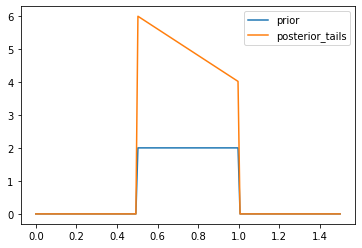
\includegraphics[width=10cm]{homework 8/homework_8_question_1b_2.png}
        \item this makes, sense as our prior, assumes that $\theta\geq.5$ but we observed a tails so our density is pushed to the left in a triangle shape
    \end{itemize}
    \item if instead we observe a heads we get 
    \begin{itemize}
        \item we know first of all that $f_{\Tilde{\theta}|\Tilde{r}}(\theta|r=1)=\frac{f_{\Tilde{\theta}}(\theta)p_{\Tilde{r}|\Tilde{\theta}}(r=1|\theta)}{p_{\Tilde{r}}(r=1)}=\frac{f_{\Tilde{\theta}}(\theta)p_{\Tilde{r}|\Tilde{\theta}}(r=1|\theta)}{\int_{u=-\infty}^{\infty} f_{\Tilde{\theta}}(u)p_{\Tilde{r=1}|\Tilde{u}}(r=1|u)du}$
        \item if $\theta<\frac{1}{2}$ or  $\theta>1$ then  $f_{\Tilde{\theta}|\Tilde{r}}(\theta|r=1)=\frac{f_{\Tilde{\theta}}(\theta)p_{\Tilde{r}|\Tilde{\theta}}(r=1|\theta)}{p_{\Tilde{r}}(r=1)}=\frac{f_{\Tilde{\theta}}(\theta)p_{\Tilde{r}|\Tilde{\theta}}(r=1|\theta)}{\int_{u=-\infty}^{\infty} f_{\Tilde{\theta}}(u)p_{\Tilde{r=1}|\Tilde{u}}(r=1|u)du}=0$
        \item if $\theta \in \{.5,1\}$then  $f_{\Tilde{\theta}|\Tilde{r}}(\theta|r=1)=\frac{f_{\Tilde{\theta}}(\theta)p_{\Tilde{r}|\Tilde{\theta}}(r=1|\theta)}{p_{\Tilde{r}}(r=1)}=\frac{f_{\Tilde{\theta}}(\theta)p_{\Tilde{r}|\Tilde{\theta}}(r=1|\theta)}{\int_{u=-\infty}^{\infty} f_{\Tilde{\theta}}(u)p_{\Tilde{r=1}|\Tilde{u}}(r=1|u)du}=\frac{(\theta)(2)}{\int_{u=\frac{1}{2}}^{1}2(u)du}=\frac{2(\theta)}{\frac{3}{4}}=\frac{8(\theta)}{3}$
              \item so our cdf looks like \\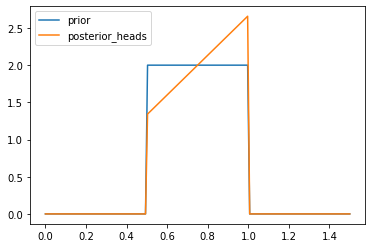
\includegraphics[width=10cm]{homework 8/homework_8_question_1b_1.png}
        \item this makes, sense as our prior, assumes that $\theta\geq.5$ but we observed a heads so our density is pushed to the the right in a triangle shape, where we assume theta is higher.
    \end{itemize}
\end{itemize}

\item You observe 100 coin flips and they all turn out to be tails (i.e. 0). Do you think you should reconsider your prior? If so, why?

\begin{itemize}
    \item yes we likely should reconsider our prior. our current prior assumes that our $\theta \geq \frac{1}{2}$ but assuming Independence, the likelihood of seeing 100 out of 100 tails flips with the lowest possible $\theta=\frac{1}{2}$ is vanishing small. 
    \item this prior would not let us update our posterior sufficiently to reflect the more likely outcome that $\theta<\frac{1}{2}$ so a difrent piror may be more reasonable
\end{itemize}
\end{enumerate}

\item (Halloween parade)
The city of New York hires you to estimate whether it will rain during the Halloween parade. Checking past data you determine that the chance of rain is 20\%. You model this using a random variable $\rnd{r}$ with pmf
\begin{align*}
 p_{\rnd{r}}(1) = 0.2, \qquad p_{\rnd{r}}(0)=0.8,
\end{align*}
where $\rnd{r}=1$ means that it rains and $\rnd{r}=0$ that it doesn't. Your first idea is to be lazy and just use the forecast of a certain website. Analyzing data from previous forecasts, you model this with a random variable $\rnd{w}$ that satisfies 
\begin{align*}
 \P(\rnd{w}=1| \rnd{r}=1) = 0.8, \qquad \P(\rnd{w}=0| \rnd{r}=0) = 0.75.
\end{align*}
\begin{enumerate}
\item What is the probability that the website is wrong?
\begin{itemize}
    \item we know that the website is wrong if $\Tilde{W}\neq \Tilde{r}$
    \item so we want $P(\tilde{w}\neq \tilde{r})=P(\Tilde{r}=1)P(\Tilde{w}=0|\title{r}=1)+P(\Tilde{r}=0)P(\Tilde{w}=1|\title{r}=0)=P(\Tilde{r}=1)(1-p(w=1|r=1))+P(\Tilde{r}=0)(1-p(w=0|r=0))=.2(.2)+.8(.25)=.24$
\end{itemize}

\end{enumerate}
Unsatisfied with the accuracy of the website, you look at the data used for the forecast (they are available online). Surprisingly the relative humidity of the air is not used, so you decide to incorporate it in your prediction in the form of a random variable $\rnd{h}$. 
\begin{enumerate}
 \item[(b)] Is it more reasonable to assume that $\rnd{h}$ and $\rnd{w}$ are independent, or that they are conditionally independent given $\rnd{r}$? Explain why.
 \begin{itemize}
     \item despite the fact that the website did not explicitly factor in humidity, rain is correlated both with humidity and the websites prediction, thus knowing the value of one gives you information about the other, and they can not be independent. 
     \itme on the other hand they might be conditionally independent as given it is raining or not, the level of humidity can not give more information about the websites prediction as it was not factored into their choice. 
 \end{itemize}
\end{enumerate}
You assume that $\rnd{h}$ and $\rnd{w}$ are conditionally independent given $\rnd{r}$. More research establishes that conditioned on $\rnd{r}=1$, $\rnd{h}$ is uniformly distributed between 0.5 and 0.7, whereas conditioned on $\rnd{r}=0$, $\rnd{h}$ is uniformly distributed between 0.1 and 0.6.  \begin{enumerate}
 \item[(c)] Compute the conditional pmf of $\rnd{r}$ given $\rnd{w}$ and $\rnd{h}$. Use the distribution to determine whether you would predict rain for any possible value of $\rnd{w}$ and $\rnd{h}$.
 \begin{itemize}
     \item so we are looking for $P_{\tilde{r}|\tilde{w},\tilde{h}}(r|w,h)=\frac{P_{\tilde{r},\tilde{w},\tilde{h}}(r,w,h)}{P_{\tilde{w},\tilde{h}}(w,h)}=\frac{P_{\tilde{h}\tilde{r}}(h|r)P_{\tilde{w}\tilde{r}}(w|r)P_{\tilde{r}}(r)}{\Sigma_{r=0}^{1}P_{\tilde{w},\tilde{h}\tilde{r}}(w,h,r)}=\\\frac{P_{\tilde{h}\tilde{r}}(h|r)P_{\tilde{w}\tilde{r}}(w|r)P_{\tilde{r}}(r)}{\Sigma_{r=0}^{1}P_{\tilde{h}\tilde{r}}(h|r)P_{\tilde{w}\tilde{r}}(w|r)P_{\tilde{r}}(r)}$
     \item so now we need to start thinking about w,h values. 
     \item consider w=1,r=1,$\tilde{h}\in\{.6,.7\}$
     \item $P_{\tilde{r}|\tilde{w},\tilde{h}}=\frac{P_{\tilde{h}\tilde{r}}(h|r)P_{\tilde{w}\tilde{r}}(w|r)P_{\tilde{r}}(r)}{\Sigma_{r=0}^{1}P_{\tilde{h}\tilde{r}}(h|r)P_{\tilde{w}\tilde{r}}(w|r)P_{\tilde{r}}(r)}=1$
     \item consider w=0,r=1,$\tilde{h}\in\{.6,.7\}$
     \item $P_{\tilde{r}|\tilde{w},\tilde{h}}=\frac{P_{\tilde{h}\tilde{r}}(h|r)P_{\tilde{w}\tilde{r}}(w|r)P_{\tilde{r}}(r)}{\Sigma_{r=0}^{1}P_{\tilde{h}\tilde{r}}(h|r)P_{\tilde{w}\tilde{r}}(w|r)P_{\tilde{r}}(r)}=1$
     \item consider w=1,r=0,$\tilde{h}\in\{.6,.7\}$
     \item $P_{\tilde{r}|\tilde{w},\tilde{h}}=\frac{P_{\tilde{h}\tilde{r}}(h|r)P_{\tilde{w}\tilde{r}}(w|r)P_{\tilde{r}}(r)}{\Sigma_{r=0}^{1}P_{\tilde{h}\tilde{r}}(h|r)P_{\tilde{w}\tilde{r}}(w|r)P_{\tilde{r}}(r)}=0$
     \item consider w=0,r=0,$\tilde{h}\in\{.6,.7\}$
     \item $P_{\tilde{r}|\tilde{w},\tilde{h}}=\frac{P_{\tilde{h}\tilde{r}}(h|r)P_{\tilde{w}\tilde{r}}(w|r)P_{\tilde{r}}(r)}{\Sigma_{r=0}^{1}P_{\tilde{h}\tilde{r}}(h|r)P_{\tilde{w}\tilde{r}}(w|r)P_{\tilde{r}}(r)}=0$
          \item consider w=1,r=0,$\tilde{h}\in\{.1,.5\}$
     \item $P_{\tilde{r}|\tilde{w},\tilde{h}}=\frac{P_{\tilde{h}\tilde{r}}(h|r)P_{\tilde{w}\tilde{r}}(w|r)P_{\tilde{r}}(r)}{\Sigma_{r=0}^{1}P_{\tilde{h}\tilde{r}}(h|r)P_{\tilde{w}\tilde{r}}(w|r)P_{\tilde{r}}(r)}=1$
     \item consider w=0,r=0,$\tilde{h}\in\{.1,.5\}$
     \item $=1$
     
     \item Consider w=0,r=1,$\tilde{h}\in\{.1,.5\}$
     \item $=0$
     
     \item consider w=1,r=1,$\tilde{h}\in\{.1,.5\}$
     \item $P_{\tilde{r}|\tilde{w},\tilde{h}}=\frac{P_{\tilde{h}\tilde{r}}(h|r)P_{\tilde{w}\tilde{r}}(w|r)P_{\tilde{r}}(r)}{\Sigma_{r=0}^{1}P_{\tilde{h}\tilde{r}}(h|r)P_{\tilde{w}\tilde{r}}(w|r)P_{\tilde{r}}(r)}=0$
     \item consider w=1,r=1,$\tilde{h}\in\{.5,.6\}$
     \item $P_{\tilde{r}|\tilde{w},\tilde{h}}=\frac{P_{\tilde{h}\tilde{r}}(h|r)P_{\tilde{w}\tilde{r}}(w|r)P_{\tilde{r}}(r)}{\Sigma_{r=0}^{1}P_{\tilde{h}\tilde{r}}(h|r)P_{\tilde{w}\tilde{r}}(w|r)P_{\tilde{r}}(r)}=\frac{2}{3}$
     \item consider w=1,r=0,$\tilde{h}\in\{.5,.6\}$
     \item $P_{\tilde{r}|\tilde{w},\tilde{h}}=\frac{P_{\tilde{h}\tilde{r}}(h|r)P_{\tilde{w}\tilde{r}}(w|r)P_{\tilde{r}}(r)}{\Sigma_{r=0}^{1}P_{\tilde{h}\tilde{r}}(h|r)P_{\tilde{w}\tilde{r}}(w|r)P_{\tilde{r}}(r)}=\frac{2(.25)(.8)}{2(.25)(.8)+2(.8)(.5)}=\frac{1}{3}$
     \item consider w=0,r=1,$\tilde{h}\in\{.5,.6\}$
     \item $P_{\tilde{r}|\tilde{w},\tilde{h}}=\frac{P_{\tilde{h}\tilde{r}}(h|r)P_{\tilde{w}\tilde{r}}(w|r)P_{\tilde{r}}(r)}{\Sigma_{r=0}^{1}P_{\tilde{h}\tilde{r}}(h|r)P_{\tilde{w}\tilde{r}}(w|r)P_{\tilde{r}}(r)}=\frac{5(.2)(.2)}{5(.2)(.2)+2(.75)(.8)}=\frac{1}{7}$
     \item consider w=0,r=0,$\tilde{h}\in\{.5,.6\}$
     \item $P_{\tilde{r}|\tilde{w},\tilde{h}}=\frac{P_{\tilde{h}\tilde{r}}(h|r)P_{\tilde{w}\tilde{r}}(w|r)P_{\tilde{r}}(r)}{\Sigma_{r=0}^{1}P_{\tilde{h}\tilde{r}}(h|r)P_{\tilde{w}\tilde{r}}(w|r)P_{\tilde{r}}(r)}=\frac{.8(2)(.75)}{.8(2)(.75)+5(.2)(.2)}=\frac{6}{7}$
     \item we can determine that we would predict rain if $P(\tilde{r}=1|\tilde{w}=w,\tilde{h}\in\mathcal{I}) \geq P(\tilde{r}=0|\tilde{w}=w,\tilde{h}\in\mathcal{I})$ and predict no rain otherwise
     
     
 \end{itemize}
 
 
 
\item[(d)] What is the probability that you make a mistake?
\begin{itemize}
    \item it would make sense to me that $P(wrong)=\frac{1}{7}(0.25*2*.8+.8*5*.2)+\frac{1}{3}(.25+2*.8+.8*5*.2)$ would be our errir rate 
    
\end{itemize}
\end{enumerate}

\item (Mixture model with fixed mean) Let $\rnd{d}$ be a Bernoulli random variable with parameter $\theta$ and let $\rnd{c}$ be a continuous random variable defined on the same probability space. The conditional distributions of $\rnd{c}$ given $\rnd{d}=0$ and $\rnd{d}=1$ are both Gaussian with zero mean and standard-deviation parameters $\sigma_0$ and $\sigma_1$ respectively. Derive the conditional pmf of $\rnd{d}$ given $\rnd{c}$. Plot $p_{\rnd{d} \cnd \rnd{c}}(1 \cnd c) $ as a function of $c$ for $\theta:=0.5$, $\sigma_0:=1$, and $\sigma_1:=0.5$.


\begin{itemize}
    \item generally we can express this as $P_{\tilde{d}|\tilde{c}}(d|c)=\frac{f_{\tilde{d}|\tilde{c}}(d|c)p_{\tilde{d}}(d)}{\Sigma_{d=0}^{1}f_{\tilde{d}|\tilde{c}}(d|c)p_{\tilde{d}(d)}}$
    \item first lets consider the case where d=0
    $P_{\tilde{d}|\tilde{c}}(d=0|c)=\frac{f_{\tilde{d}|\tilde{c}}(d=0|c)p_{\tilde{d}}(d=0)}{\Sigma_{d=0}^{1}f_{\tilde{d}|\tilde{c}}(d|c)p_{\tilde{d}(d)}}=\\\frac{(1-\theta)\frac{1}{\sqrt{2\pi}\sigma_{0}}e^{-\frac{1}{2}(\frac{C}{\sigma_0})^{2}}}{(1-\theta)\frac{1}{\sqrt{2\pi}\sigma_{0}}e^{-\frac{1}{2}(\frac{C}{\sigma_0})^{2}}+(\theta)\frac{1}{\sqrt{2\pi}\sigma_{1}}e^{-\frac{1}{2}(\frac{C}{\sigma_1})^{2}}}=\frac{1}{1+\frac{\theta}{1-\theta}\frac{\sigma_0}{\sigma_1}e^{\frac{1}{2}(\frac{c}{\sigma_0})^2-\frac{1}{2}(\frac{c}{\sigma_1})^2}}$
    \item next consider where d=1
    $P_{\tilde{d}|\tilde{c}}(d=1|c)=\frac{f_{\tilde{d}|\tilde{c}}(d=1|c)p_{\tilde{d}}(d=1)}{\Sigma_{d=0}^{1}f_{\tilde{d}|\tilde{c}}(d|c)p_{\tilde{d}(d)}}=\\\frac{(\theta)\frac{1}{\sqrt{2\pi}\sigma_{1}}e^{-\frac{1}{2}(\frac{C}{\sigma_1})^{2}}}{(1-\theta)\frac{1}{\sqrt{2\pi}\sigma_{0}}e^{-\frac{1}{2}(\frac{C}{\sigma_0})^{2}}+(\theta)\frac{1}{\sqrt{2\pi}\sigma_{1}}e^{-\frac{1}{2}(\frac{C}{\sigma_1})^{2}}}=\frac{1}{1+\frac{1-\theta}{\theta}\frac{\sigma_1}{\sigma_0}e^{\frac{1}{2}(\frac{c}{\sigma_1})^2-\frac{1}{2}(\frac{c}{\sigma_0})^2}}$
    \\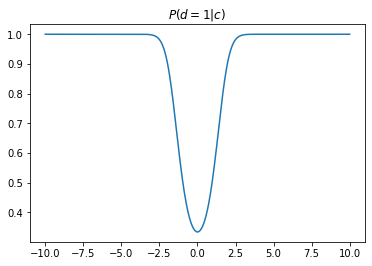
\includegraphics[width=10cm]{homework 8/homework_8_question_3.png}
\end{itemize}

\item (Breast Cancer)
A hospital is interested in developing a system for automatic breast cancer detection from the radius (mean of distances from center to points on the perimeter) and texture (standard deviation of gray-scale values) of tumors. You model whether the tumor is benign or malignant as a random variable $\rnd{c}$:
\begin{align*}
\rnd{c} = \begin{cases}
0 \quad \text{if the tumor is benign},\\
1 \quad \text{if the tumor is malignant}.
\end{cases} 
\end{align*}
The available data contain the radius and texture of each tumor. We model these quantities as the continuous random variables $\rnd{r}$ and $\rnd{t}$. Assume that the radius and texture of tumor are conditionally independent given the type of tumor (benign or malignant). 

\begin{enumerate}
\item Derive the \emph{maximum a posteriori} (MAP) estimate of $\rnd{c}$ given $\rnd{r}$ and $\rnd{t}$ as a function of the pmf of $\rnd{c}$ ($ p_{\rnd{c}}$) and the conditional pdfs $f_{\rnd{r}|\rnd{c}}$ and $f_{\rnd{t}|\rnd{c}}$. The MAP estimate is defined as the mode of the posterior pmf.

\begin{itemize}
    \item $\hat{c}=argmaxP(c|r,t)=argmax\frac{P(c,r,t)}{P(r,t)}=argmax\frac{f(r|c)f(t|c)P(c)}{f(r|c=0)f(t|c=0)P(c=0)+f(r|c=1)f(t|c=1)P(c=1)}$ as c is fixed in the denommicator the maximization problem simplfies to $\hat{c}=argmaxf(r|c)f(t|c)P(c)$
\end{itemize}


\item

Complete the corresponding part of the script \emph{breast\_cancer.ipynb} to estimate the necessary probability mass functions from the data. The training data consists of 398 patients and is provided in \emph{train\_X["mean radius"]}, \emph{train\_X["mean texture"]} and \emph{train\_y}. 
Apply the MAP decision rule you derived in part (a) to predict whether a group of 171 other patients, whose information is stored in the \emph{test\_X} and \emph{test\_y}. Experiment with parametric Gaussian models with MLE and non-parameteric models with KDE at different bandwidths to estimate $f_{\rnd{r}|\rnd{c}}$ and $f_{\rnd{t}|\rnd{c}}$ and compare the error rate on the test set.
\end{enumerate}
\begin{itemize}
    \item use parametric methods i found an erorr rate of around $14\%$
    \item using kde with a bandwith of 1 i got an error of $12\%$
    \item using kde with a bandwith of 1 i got an error of $11\%$
    \item using kde with a bandwith of 1 i got an error of $18\%$
\end{itemize}
\end{enumerate}
\end{document}
